\documentclass{beamer}
\usetheme{Rochester}

\title[F3ildCrypt]{F3ildCrypt: End-to-End Protection of Sensitive Information
in Web Services}

\author[Burnside, Keromytis]{Matthew Burnside and Angelos D. Keromytis}

\institute[Columbia University]{
Department of Computer Science\\
Columbia University\\
\texttt{\{mb, angelos\}@cs.columbia.edu}
}
\date{ISC 2009}

\begin{document}

\begin{frame}[plain]
    \titlepage
\end{frame}

\begin{frame}
\frametitle{Motivation}
\begin{itemize}
\item Identity-related information is valuable
\item You must provide such information when using an online merchant
\item This information is vulnerable to disclosure at the endpoints and in
transit 
\item Can we protect this information end-to-end without revealing details of
the logical corporate architecture?
\end{itemize}
\end{frame}

\begin{frame}
\frametitle{Outline}
\tableofcontents
\end{frame}

\section{Introduction}
\begin{frame}
\frametitle{}
\begin{center}
Introduction
\end{center}
\end{frame}

\begin{frame}
\frametitle{Merchant trust}
Users have to trust online merchants:
\smallskip
\begin{itemize}
\item Merchant is not malicious
\item Merchant will protect sensitive information for its lifetime
\item Merchant site is maintained by diligent sysadmins
\end{itemize}
\end{frame}

\begin{frame}
\frametitle{Service-oriented architecture}
In this work, we focus on SOAs:
\smallskip
\begin{itemize}
\item Requests to a network have a single entry point
\item A parent SOA may make requests on multiple child SOAs 
\item SOAs may operate under differing legal and corporate policies toward
private data
\end{itemize}
\end{frame}

\begin{frame}
\frametitle{SOA trust}
In Service Oriented Architectures, users have to trust:
\smallskip
\begin{itemize}
\item Merchant \emph{and peer SOAs} are not malicious
\item Merchant \emph{and peer SOAs} will protect sensitive information for its
lifetime
\item Merchant \emph{and peer SOAs} are maintained by diligent sysadmins
\end{itemize}
\end{frame}

\begin{frame}
\frametitle{Data in transit}
We consider only data in transit across the SOA pipeline
\smallskip
\begin{itemize}
\item We protect the data between the web browser and the back-end database
\item Our approach does not protect against nodes with legitimate access to the
data
\end{itemize}
\end{frame}

% \begin{frame}
% \frametitle{Example}
% \begin{itemize}
% \item XXX: Diagram showing web browser, merchant, and SOA doing credit-card
% transactions.  Even with SSL, only protected from web browser to merchant.
% \end{itemize}
% \end{frame}

\begin{frame}
\frametitle{Design alternative}
Pair-wise key distribution
\smallskip
\begin{itemize}
\item Generate a public key for each potential destination host in the SOA
pipeline
\item Deliver public keys to each web browser
\item Browser encrypts each field direct to its destination host 
\end{itemize}
\end{frame}

\begin{frame}
\frametitle{Design alternative (cont.)}
Issues with pair-wise key distribution
\smallskip
\begin{itemize}
\item Public keys for all hosts in any partner SOAs must also be delivered
\item Public keys must be updated each time the architecture of the SOA or
its partners varies
\item Reveals the logical architecture of the SOA and its SOA partners
\end{itemize}
\end{frame}

\section{Related work}
\begin{frame}
\frametitle{}
\begin{center}
Related work
\end{center}
\end{frame}

% \begin{frame}
% \frametitle{XACML}
% \begin{itemize}
% \item eXtensible Access Control Markup Language
% \item XML standard for defining policies, requests, and reponses
% \end{itemize}
% \end{frame}

\begin{frame}
\frametitle{Proxy re-encryption}
\begin{itemize}
\item Given plaintext $P$, Alice $\langle pk_A, sk_A \rangle$, and Bob
$\langle pk_B, sk_B \rangle$
\item There exists some $rk_{A \to B} = F(sk_A, pk_B)$ such that:
\begin{equation*}
pk_B(p) = rk_{A \to B}( pk_A (P))
\end{equation*}
\item \cite{atomic_proxy_reencryption} 
% \item \cite{proxy_reencryption}
\end{itemize}
\end{frame}

\begin{frame}
\frametitle{W3bCrypt}
Introduced end-to-end encryption in web pipelines
\smallskip
\begin{itemize}
\item \emph{``Encryption as a stylesheet''}
\item Firefox plugin for application-level crypto
\item Requires disclosure of corporate network details
\item \cite{w3bcrypt} 
\end{itemize}
\end{frame}

\section{Architecture}
\begin{frame}
\frametitle{}
\begin{center}
Architecture
\end{center}
\end{frame}

\begin{frame}
\frametitle{Architecture}
\begin{itemize}
\item Network model
\item Design goals
\item F3ieldCrypt architecture
\end{itemize}
\end{frame}

\begin{frame}
\frametitle{Network model}
\begin{itemize}
\item SOA-style network
\item Each SOA may have multiple partner SOAs
\item SOAs wish to prevent disclosure of logical architecture and peering 
\end{itemize}
\end{frame}

% \begin{frame}
% \frametitle{Threat model}
% \begin{itemize}
% \item XXX
% \end{itemize}
% \end{frame}

\begin{frame}
\frametitle{Design goals}
\begin{itemize}
\item End-to-end protection of XML fields -- even across SOA boundaries
\item Confidentiality of logical architecture of each SOA must be respected
\end{itemize}
\medskip
\small{\emph{This work does not focus on providing protection against
compromise or failure of entities with legitimate access to sensitive
information.}}
\end{frame}

\begin{frame}
\frametitle{F3ieldCrypt architecture}
\begin{itemize}
\item Each SOA $s$ publishes a public key $pk_{E_s}$
\item Browser $b$ generates plaintext $P$
\item $b$ sends $C = pk_{E_s}(P)$ to $s$
\item Gateway at $s$ re-encrypts $C$ to internal hosts and partner SOAs
$I_0...I_n$ 
\end{itemize}
\end{frame}

\begin{frame}
\frametitle{Key generation}
\begin{itemize}
\item Key pair $\langle pk_{E_s}, sk_{E_s} \rangle$ generated at the
\alert{external-key holder}
% \item SOA collects the public keys of its applications $pk_{I_0}...pk_{I_n}$
\item $sk_{E_s}$ used in conjunction with internal application keys
$pk_{I_0}...pk_{I_n}$ to generate $rk_{E \to I_0}...rk_{E \to I_n}$
\end{itemize}
\end{frame}

\begin{frame}
\frametitle{External-key holder}
External-key holder has $sk_s$ and $pk_{I_0}...pk_{I_n}$ --- its compromise
could be dangerous.  However:
\smallskip
\begin{itemize}
\item Very low bandwidth requirements
\item Only needed at setup and when adding new internal hosts
\item Can be kept offline!
\end{itemize}
\end{frame}

\begin{frame}
\frametitle{Key distribution}
\begin{itemize}
\item $pk_{E_s}$ is publicized
\item $rk_{E \to I_0}...rk_{E \to I_n}$ transmitted to \alert{proxy
re-encryption engine}
\item By proxy re-encryption:
\begin{equation*}
pk_{I_j}(P) = rk_{E \to I_j}( pk_E (P))
\end{equation*}
\end{itemize}
\end{frame}

\begin{frame}
\frametitle{Proxy re-encryption engine}
\begin{itemize}
\item Fields arrive at proxy re-encryption engine encrypted under $pk_{E_s}$
\item Each field $f$ is re-encrypted to $pk_{I_j}$
\item The mapping $f \to j$ is determined by an admin-defined XACML policy
\end{itemize}
\end{frame}

\begin{frame}
\frametitle{Browser engine}
\begin{itemize}
\item \alert{Browser} generates plaintext $P$ containing a set of fields
$f_0...f_n$
\item $f_0...f_n$ are encrypted under $pk_{E_s}$ and delivered to $s$
\end{itemize}
\end{frame}

% \begin{frame}
% \frametitle{Client policy and crypto engines}
% Web clients receive a re-cryptography engine and a policy engine. 
% \medskip
% \begin{itemize}
% \item \alert{Policy engine} uses a XACML policy to determine which fields to
% encrypt
% \item \alert{Re-crypto engine} encrypts XML fields as directed by the policy
% engine.
% \end{itemize}
% \end{frame}

\begin{frame}
\frametitle{Architecture summary}
% \begin{center}
\begin{tabular}{ll}
browser $\to$ proxy re-encryption engine: & $pk_{E_s}(f_i)$ \\
proxy re-encryption engine: & $pk_{I_j}(f_i) = rk_{E \to I_j}(pk_{E_s}(f_i))$ \\
proxy re-encryption engine $\to$ app $j$: & $pk_{I_j}(f_i)$ \\
\end{tabular}
% \end{center}
\end{frame}

\section{Evaluation}
\begin{frame}
\frametitle{}
\begin{center}
Evaluation
\end{center}
\end{frame}

\begin{frame}
\frametitle{Implementation}
\begin{itemize}
\item Java-based Re-crypto engine uses JHU-MIT Proxy Re-cryptography Library
for each browser 
\item XML gateway at the SOA stores the re-encryption engine 
\item Python-based XML proxy for each internal application to store keys and
unwrap XML
\end{itemize}
\end{frame}

\begin{frame}
\frametitle{Testbed servers}
Dell PowerEdge 2650 Servers
\begin{itemize}
\item 2.0GHz Intel Zeon processor, 1GB RAM, Gigabit Ethernet
\item OpenBSD 4.2
\item OpenBSD PF firewall, Apache 1.3.29, PHP 4.4.1, MySQL 5.0.45 
\end{itemize}
\end{frame}

\begin{frame}
\frametitle{Testbed client}
Macbook Pro
\begin{itemize}
\item 2.4 GHz Intel Core 2 Duo, 2GB RAM, Gigabit Ethernet
\item OS X 10.5.2, Darwin kernel 9.2.2, Mozilla Firefox 2.0.0.13
\end{itemize}
\end{frame}

\begin{frame}
\frametitle{Block encryption on the client}
\begin{center}
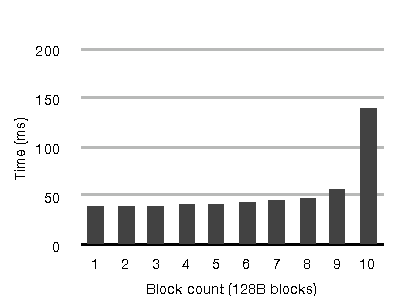
\includegraphics{client_field_count_new} \\
\end{center}
\end{frame}

\begin{frame}
\frametitle{Re-encryption rate at an XML gateway}
\begin{center}
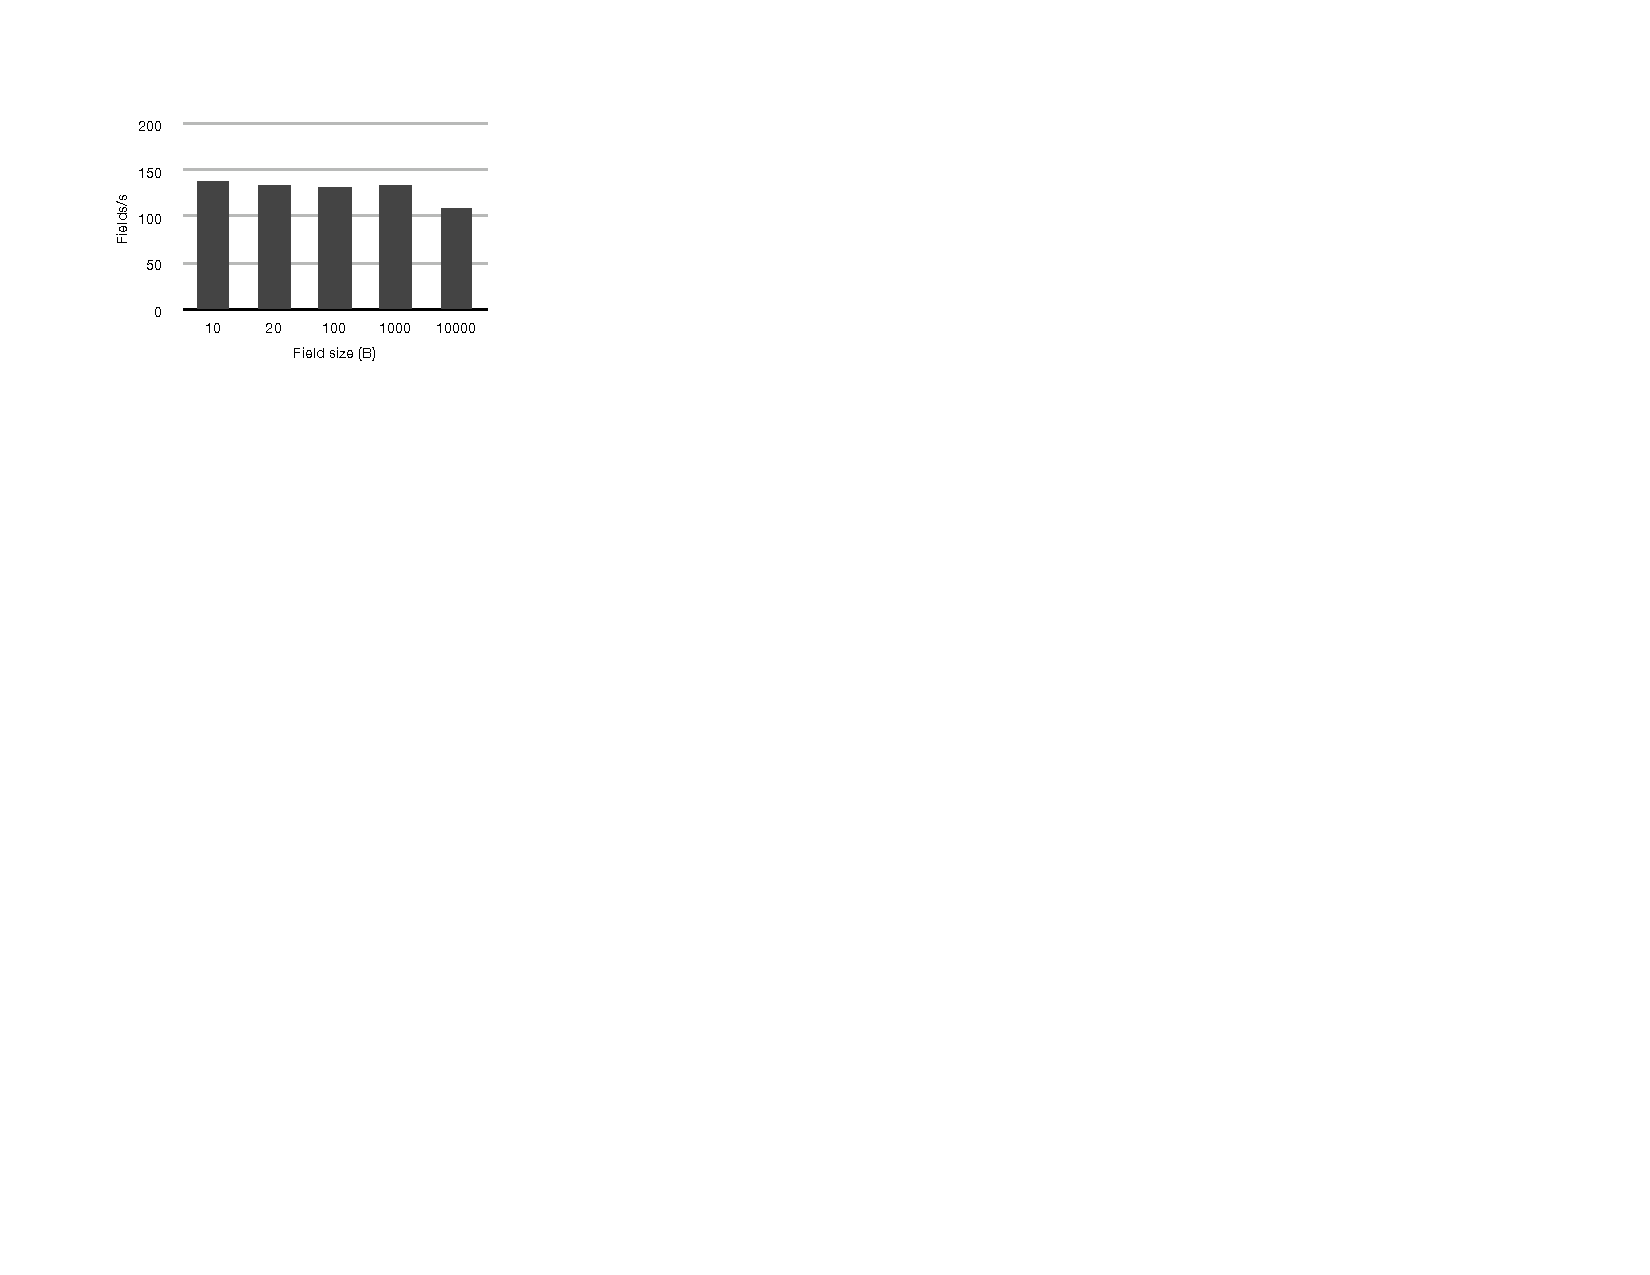
\includegraphics{server_encrypt} \\
\end{center}
\end{frame}

\begin{frame}
\frametitle{Decryption rate at an XML proxy}
\begin{center}
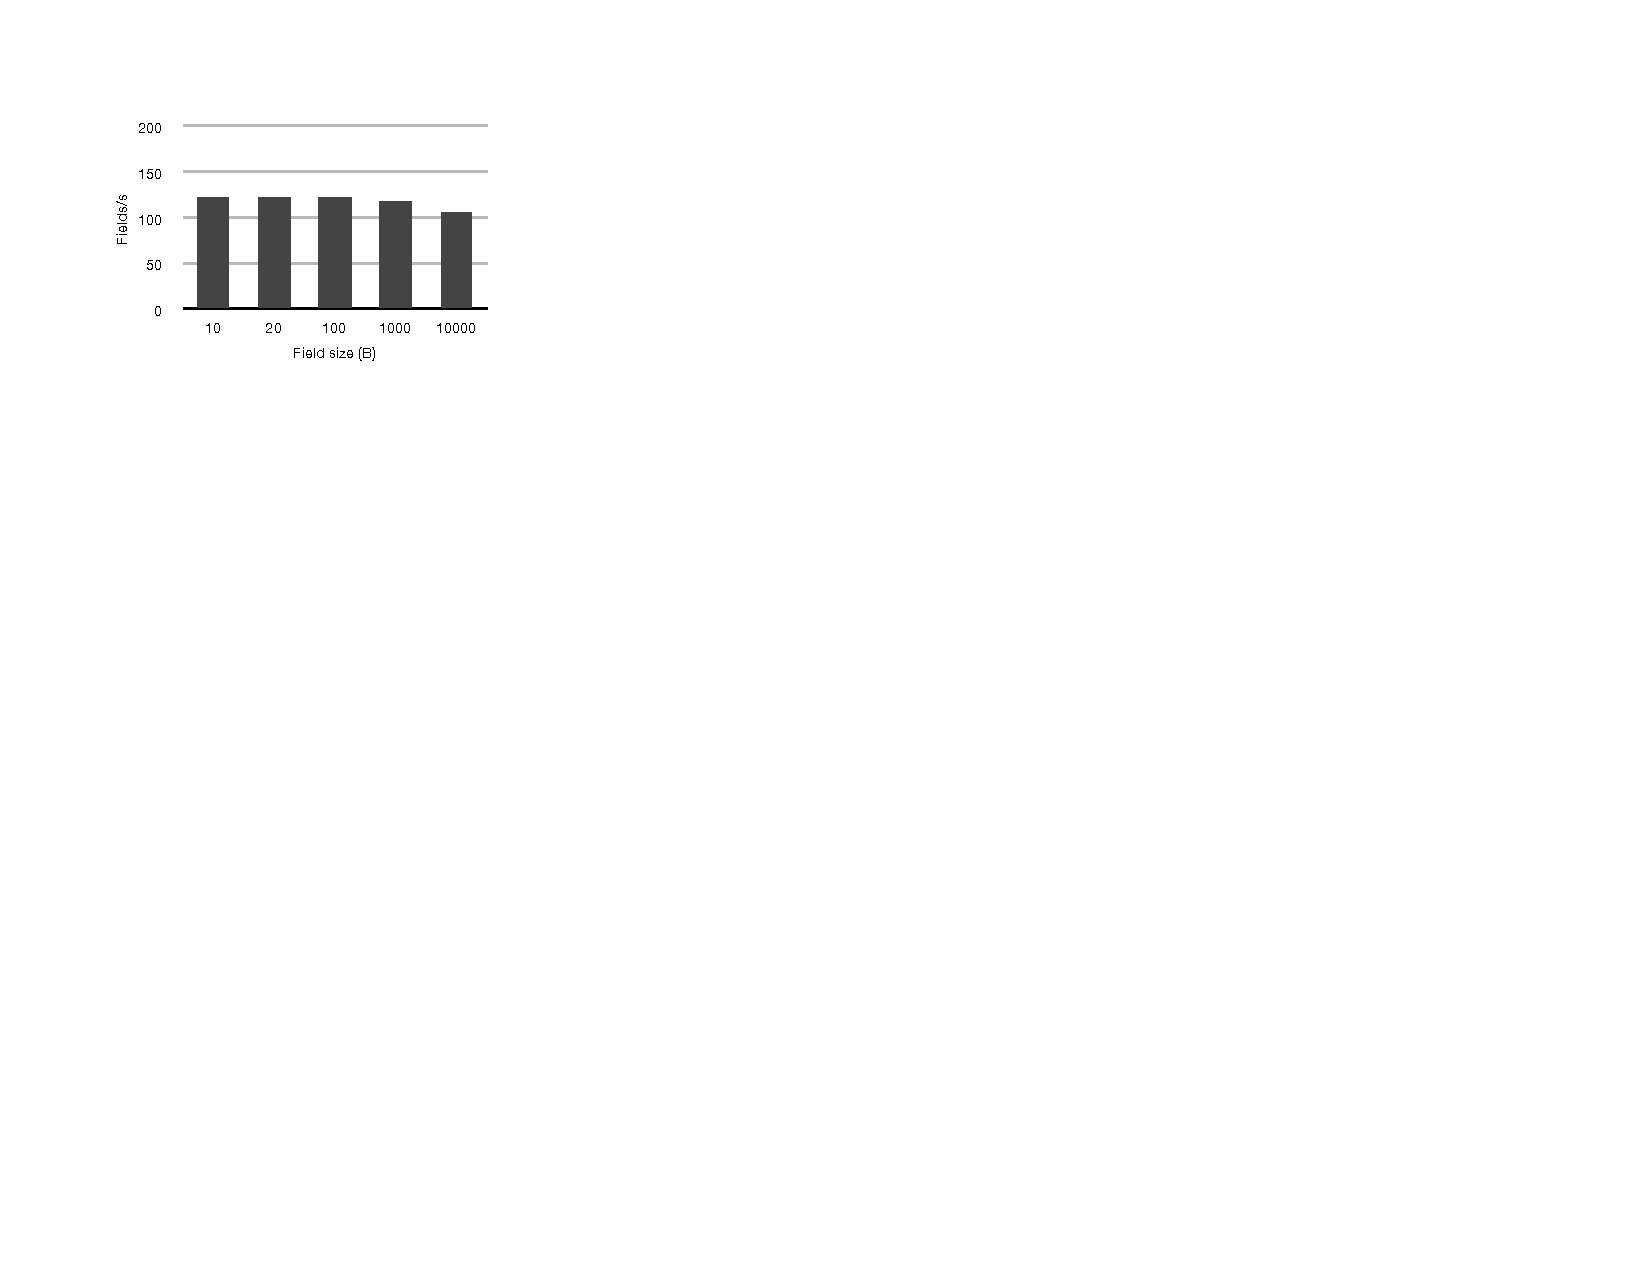
\includegraphics{server_decrypt} \\
\end{center}
\end{frame}

\section{Conclusion}
\begin{frame}
\frametitle{Conclusion}
\begin{itemize}
\item End-to-end protection to users 
\item Protection of logical architecture and partnering for SOAs
\end{itemize}
\end{frame}

\begin{frame}
\frametitle{References}
\begin{thebibliography}{10}
% \bibitem[Ateniese et al., 2005]{proxy_reencryption}
% G.~Ateniese, K.~Fu, M.~Green, and S.~Hohenberger.
% \newblock Improved proxy re-encryption schemes with applications to secure
%   distributed storage.
% \newblock In {\em Proceedings of the 12th Annual Network and Distributed
%   Systems Security Symposium (NDSS 2005)}, 2005.

\bibitem[Blaze et al., 1998]{atomic_proxy_reencryption}
Matt Blaze, G.~Bleumer, and M.~Strauss.
\newblock Divertible protocols and atomic proxy cryptography.
\newblock In {\em Proceedings of Eurocrypt '98}, pages 127--144, 1998.

\bibitem[Stavrou et al., 2006]{w3bcrypt}
Angelos Stavrou, Michael Locasto, and Angelos Keromytis.
\newblock W3bcrypt: Encryption as a stylesheet.
\newblock In {\em Proceedings of the 4th Applied Cryptography and Network
  Security Conference (ACNS 2006)}, pages 349--364, 2006.
\end{thebibliography}
\end{frame}


\end{document} 
